% -*- mode: latex; mode: auto-fill; coding: utf-8; -*-

\chapter{Constructing Volumetric Meshes}
\label{sec:constructing-meshes}
Suppose that we have constructed the model shown in figure \vref{fig:bar5}
(repeated below in figure \ref{fig:bar5-repeaded}), and want to
convert this model into a volumetric mesh for use in the simulator.

\begin{figure}
  \centering
  \subfloat[bar $5 \times 5 \times 5$.]{
    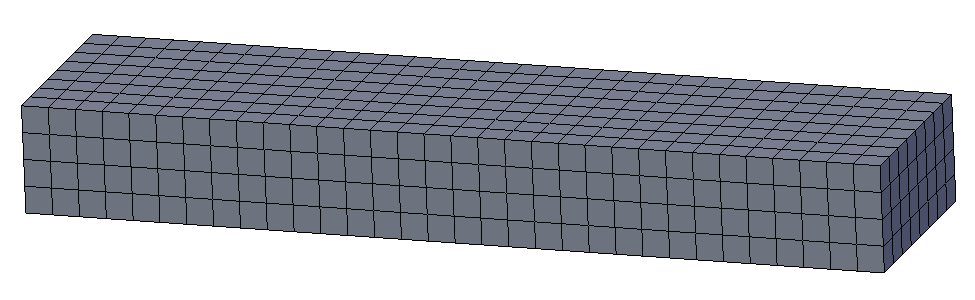
\includegraphics[width=7cm]{./images/appendix_test_data_bar_5.png}
    \label{fig:bar5-repeaded}
  }
  \subfloat[bar $5 \times 5 \times 5$ triangularized.]{
    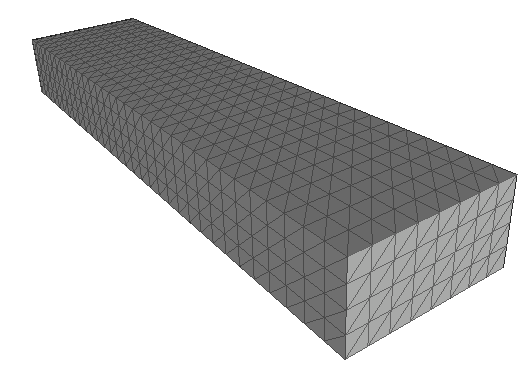
\includegraphics[width=7cm]{./images/appendix_surface_model_bar5_triangulized.png}
    \label{fig:bar5-triangularized}
  }
  \caption{The bar $5 \times 5 \times 5$ as quadratic and triangularized
    surface mesh.}
  \label{fig:bar}
\end{figure}

To export this surface mesh from Blender and hereby triangularize it,
as illustrated in figure \vref{fig:bar5-triangularized}, choose the
following from the menu inside Blender (tested on Blender version 2.48a):
[File] $\rightarrow$ [Export], and choose the [Stanford PLY] format. \\

\code{output from Blender: bar5x5x5.ply} \\

Open this file with MeshLab (tested with version 1.2.2) and convert
the file using the menu items: [File] $\rightarrow$ [Save as...]. A
dialog appears, choose the [STL File Format]. In the next dialog
uncheck the checkbox named ``Binary encoding''. It is importent to
uncheck this checkbox because TetGen only accepts ASCII files as input. \\

\code{output from MeshLab: bar5x5x5.stl} \\

Generate the volumetric body mesh using TetGen (tested with
version 1.4.2), which is a command line tool. Enter the following into
the command line: \\

\code{./tetgen -pqAzF bar5x5x5.stl} \\

\code{output from TetGen: bar5x5x5.1.ele, bar5x5x5.1.node, and bar5x5x5.1.smesh}\\

the \code{.node} files contains a vertex-pool, the \code{.ele} the
body mesh, and the \code{.smesh} the surface mesh, as described in
section \vref{sec:data-model}. It is these three files we load into our
program.
Note that the number of surface triangles generated by TetGen from the
original surface model, is a order of magnitude larger than in the
original model. This is caused by Blender's way of triangularizing the
surface, which does not take into account that we, as a final goal, want
to generate a volumetric mesh.
\\

The applications used are all cross platform and open source
applications and can be downloaded from the following web sites:
\url{http://www.blender.org/},
\url{http://meshlab.sourceforge.net/}, and
\url{http://tetgen.berlios.de/}.
